\chapter{\textit{Teori}}
\section{Sejarah \textit{Python}}
\par Python adalah bahasa pemrograman interpretatif multiguna dengan filosofi perancangan yang berfokus pada tingkat keterbacaan kode.Python diklaim sebagai bahasa yang menggabungkan kapabilitas, kemampuan, dengan sintaksis kode yang sangat jelas,dan dilengkapi dengan fungsionalitas pustaka standar yang besar serta komprehensif. Python juga didukung oleh komunitas yang besar.

\par Python mendukung multi paradigma pemrograman, utamanya; namun tidak dibatasi; pada pemrograman berorientasi objek, pemrograman imperatif, dan pemrograman fungsional. Salah satu fitur yang tersedia pada python adalah sebagai bahasa pemrograman dinamis yang dilengkapi dengan manajemen memori otomatis. Seperti halnya pada bahasa pemrograman dinamis lainnya, python umumnya digunakan sebagai bahasa skrip meski pada praktiknya penggunaan bahasa ini lebih luas mencakup konteks pemanfaatan yang umumnya tidak dilakukan dengan menggunakan bahasa skrip. Python dapat digunakan untuk berbagai keperluan pengembangan perangkat lunak dan dapat berjalan di berbagai platform sistem operasi.
\section{Sejarah \textit{Selenium}}
Kisah ini dimulai pada 2004 di ThoughtWorks di Chicago, dengan Jason Huggins membangun mode Inti sebagai JavaScriptTestRunner untuk pengujian aplikasi waktu dan Pengeluaran internal (Python, Plone). Pengujian otomatis terhadap aplikasi apa pun adalah inti dari gaya ThoughtWork, mengingat kecenderungan Agile dari konsultasi ini. Dia mendapat bantuan dari Paul Gross dan Jie Tina Wang. Bagi mereka, ini adalah pekerjaan harian.

Jason mulai memperagakan alat uji ke berbagai rekan. Banyak yang senang dengan umpan balik visual yang langsung dan intuitif, serta potensinya untuk tumbuh sebagai kerangka pengujian yang dapat digunakan kembali untuk aplikasi web lainnya.

Segera setelah tahun 2004 sesama ThoughtWorker Paul Hammant melihat demo, dan memulai diskusi tentang sumber terbuka Selenium, serta mendefinisikan mode 'didorong' Selenium di mana Anda bisa menggunakan Selenium melalui kabel dari bahasa pilihan Anda. , yang akan menyiasati 'kebijakan asal yang sama'. Rekan-rekan (saat itu) lainnya, Aslak Hellesoy dan Mike Melia, bereksperimen dengan berbagai ide untuk karya 'server', termasuk penulisan ulang halaman untuk mendapatkan kebijakan asal yang sama. Paul menulis karya server asli di Jawa, dan Aslak dan Obie Fernandez mengangkut driver klien ke Ruby, menetapkan fondasi untuk driver dalam lebih banyak bahasa.

Pekerja Pikir di berbagai kantor di seluruh dunia mengambil Selenium untuk proyek komersial, dan berkontribusi kembali ke Selenium dari pelajaran yang dipetik dari proyek ini. Mike Williams, Darrell Deboer, dan Darren Cotterill semuanya membantu meningkatkan kemampuan dan ketahanannya.

\section{Jenis-Jenis \textit{Selenium} \textit{}}
Selenium adalah perangkat lunak yang berfungsi untuk mendukung pengembangan otomatisasi uji berbasis web aplikasi. Selenium menyediakan pengujian khusus terhadap domain bahasa,untuk melakukan tes menulis pada beberapa bahasa pemrograman yan populer, termasuk C, Groovy, Java, Pearl, PHP, Python, Ruby, dan juga Scala. Pengujian dapat berjalan melalui browser web apa saja dan dapat dilakukan melalui Sistem Operasi di Windows, Linux, dan Platform OS X. Selenium Python Bindings menyediakan API yang sederhana untuk menulis uji fungsional menggunakan Selenium WebDriver, dan juga dapat mengakses semua fungsi Selenium WebDriver secara intuitif. Selenium Python Bindings menyediakan API yang cukup nyaman untu melakukan suatu akses Selenium WebDrivers seperti di Firefox, Internet Explorer, Chrome, dll 

Jenis-Jenis Selenium Sebagai Berikut :

\begin{enumerate}

\item \textit{IDE selenium}
\par Selenium IDE (Lingkungan Pengembangan Terpadu) adalah sumber terbuka alat rekam dan putar untuk menghasilkan skrip Selenium, yang terintegrasi dengan browser web Firefox sebagai ekstensi. Ini adalah tes UI berbasis web yang terkenal alat otomatisasi yang mengekstrak segala jenis locator dari halaman web. Ator banyak yang bisa baik berbasis atribut atau berbasis struktur, dan termasuk ID, nama, tautan, XPath, CSS, dan DOM. IDE memiliki seluruh Selenium Core, yang memungkinkan pengguna mencatat 10, memutar, mengedit, dan men-debug tes secara manual di browser. Tindakan pengguna di web halaman dapat direkam dan diekspor dalam bahasa apa saja yang paling populer, seperti Java, C , Ruby, dan Python, Selenium Builder adalah alat open source alternatif untuk dicatat oleh Selenium IDE dan pemutaran aplikasi web. Ini adalah ekstensi dari web browwr Firefox, Yang mirip dengan Selenium IDE, tetapi, ia memiliki beberapa fitur unik yaitu Selenium IDE tidak mendukung. S'lenium Builder adalah alat standar dari Sauce Lahs yang menjalankan tes Sauce Cloud dari antarmuka Selenium Builder itu sendiri.

\item \textit{Selenium WebDriver}
\par Selenium webdriver adalah versi terbaru dari selenium IDE dan selenium Remote Control (RC). Ini juga dinamai selenium 2.0. Ini memungkinkan skrip uji yang dirancang untuk berkomunikasi dengan browser secara langsung dengan bantuan metode asli. Ini mendukung pengujian aplikasi web pada desktop serta pada perangkat seluler seperti Android dan iOS
perangkat. Biaya proyek berkurang dengan bantuan ini alat karena itu adalah alat open-source. Waktu yang diperlukan untuk mengeksekusi skrip pengujian di webdriver kurang jika dibandingkan ke selenium IDE dan Selenium RC.Ini memungkinkan skrip pengujian dirancang untuk berbagai browser seperti Internet explorer, Firefox, Mac safari dan Chrome. Script pengujian dapat dikembangkan menggunakan bahasa seperti Java, C , Ruby, Perl, Python.


\item \textit{Remote Control Selenium}
\par Remote Control Selenium (RC) adalah selenium utama yang digunakan untuk memproyeksikan waktu yang lama. Selenium RC lebih lambat daripada selenium webdriver karena menggunakan program java script yang disebut sebagai suatu inti dari selenium. Selenium RC harus memulai server sebelum menjalankan suatu skrip pengujian, dan itu tidak mendukung untuk aplikasi Ajax. Cara menghindari keterbatasan Selenium RC, aitu dengan selenium Web Driver.

\item \textit{Selenium Grid}
\par Server yang memungkinkan pengujian untuk menggunakan instace browser web yang sedang berjalan di mesin jarak jauh. Dengan selenium grid, satu server bertindak sebagai hub. Tes hubungi hub untuk mendapatkan akses ke instance browser karena hub memiliki daftar server yang menyediakan akses ke insntance browser (node WebDriver), dan memungkinkan pengujian menggunakan instance ini. Selenium Grid memiliki kemampuan untuk menjalankan tes pada instance browser jarak jauh yang berguna untuk menyebarkan beban pengujian di beberapa mesin, dan untuk menjalankan tes di browser yang berjalan pada platform atau sistem operasi yang berbeda. Yang terakhir ini sangat berguna dalam kasus di mana tidak semua browser yang akan digunakan untuk pengujian dapat berjalan pada platform yang sama.

\item \textit{TestNG} 
\par TestNG adalah kerangka pengujian yang digunakan untuk pengujian otomatisasi bersama dengan selenium 2.0.Ini mendukung berbagai tingkat pengujian seperti unit, integrasi, sistem dan pengujian penerimaan pengguna (UAT). Biasanya disebut sebagai"Uji Generasi Baru".
\end{enumerate}

\section{Anaconda}
Distribusi open-source Anaconda adalah cara termudah untuk melakukan sains data Python / R dan pembelajaran mesin di Linux, Windows, dan Mac OS X. Dengan lebih dari 15 juta pengguna di seluruh dunia, ini adalah standar industri untuk pengembangan, pengujian, dan pelatihan tentang mesin tunggal,

\subsection{Instalasi Anaconda}
Hal yang harus diperhatikan sebelum melakukan instalasi \textit{Anaconda Python}
\begin{enumerate}
 \item Perhatikan versi dari sistem operasi yang digunakan (versi 32bit atau 64bit)
 \item Download file anaconda yang sesuai dengan versi sistem operasi (32bit atau 64bit)
 \item \textit{Download Anaconda Python} https://www.anaconda.com/distribution/
\end{enumerate}

Berikut langkah-langkah instalasi anaconda.
\begin{enumerate}
\item Buka aplikasi \textit{installer Anaconda} tersebut lalu akan muncul  gambar \textit{installer anaconda}.
\begin{figure}[H]
        \centerline{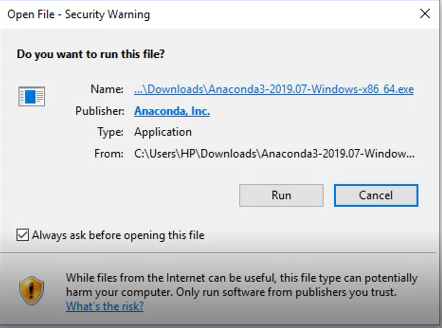
\includegraphics[scale=0.5]{figures/1}}
        \caption{Run Setup Anaconda}
		\label{langkah1}
\end{figure}

\item Tunggu hingga \textit{setup loading} selesai
\begin{figure}[H]
        \centerline{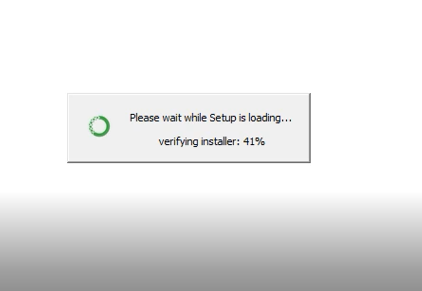
\includegraphics[scale=0.5]{figures/2}}
        \caption{Setup Loading}
		\label{langkah2}
\end{figure}


\item Jika \textit{setup loading} telah selesai, maka klik \textit{next}
\begin{figure}[H]
        \centerline{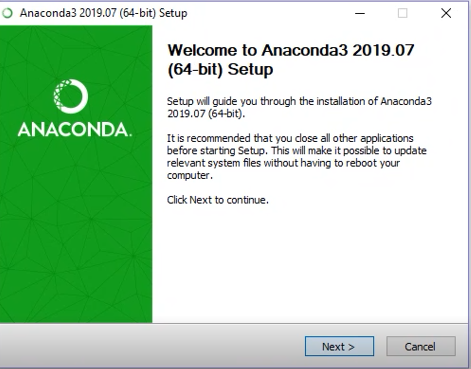
\includegraphics[scale=0.5]{figures/3}}
        \caption{Welcome to Anaconda Setup}
		\label{langkah2}
\end{figure}


\item Pada \textit{License Agreement} klik \textit{I Agree}
 gambar \textit{License Agreement}.

\begin{figure}[H]
    \centering
    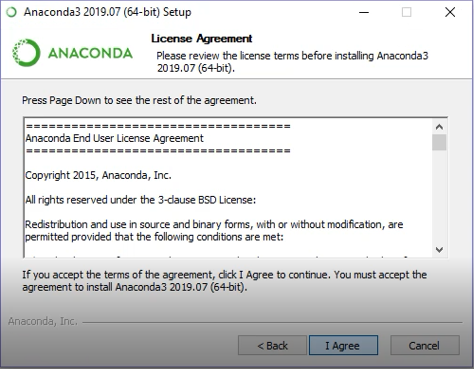
\includegraphics[scale=0.5]{figures/4}
    \caption{\textit{License Agreement}}
    \label{Figureanaconda3}
\end{figure}


\item Kemudian pilih \textit{Just Me(Recomended)} agar sesuai dengan komputer yang digunakan, kemudian klik \textit{next}
 gambar \textit{Just Me(recomended)}.

\begin{figure}[H]
    \centering
    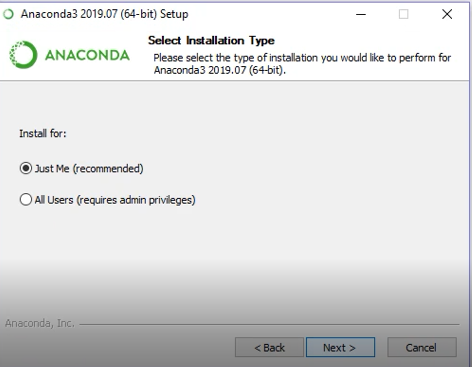
\includegraphics[scale=0.5]{figures/5}
    \caption{\textit{Just Me(recomended)}}
    \label{Figureanaconda4}
\end{figure}


\item Kemudian pilih lokasi tempat \textit{menginstall anaconda}
 gambar \textit{Pilih lokasi}.

\begin{figure}[H]
    \centering
    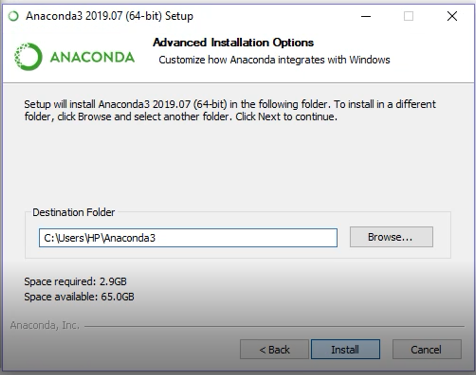
\includegraphics[scale=0.5]{figures/6}
    \caption{\textit{Pilih lokasi}}
    \label{Figureanaconda5}
\end{figure}

\item Kemudian centang \textit{Add Anaconda to my Path environtment variable}, agar saat \textit{menginstall selenium} langsung ke \textit{path anaconda} tidak ke aplikasi yang lain. Klik \textit{install}
 gambar \textit{Centang Anaconda to my PATH}.

\begin{figure}[H]
    \centering
    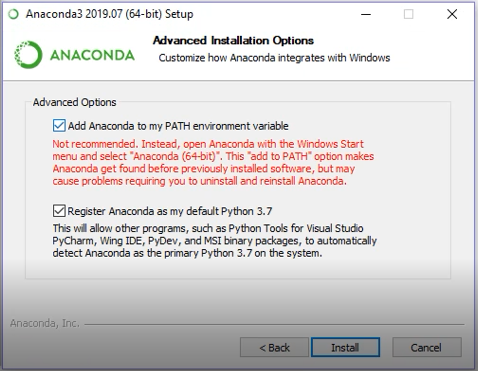
\includegraphics[scale=0.5]{figures/7}
    \caption{\textit{Centang Anaconda to my PATH}}
    \label{Figureanaconda6}
\end{figure}

\item Tunggu sampai proses \textit{installasi} selesai
 gambar \textit{Installation Complete}.

\begin{figure}[H]
    \centering
    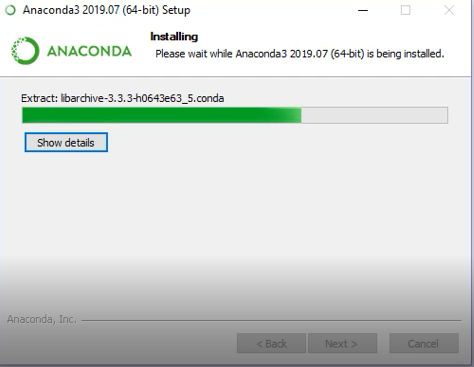
\includegraphics[scale=0.5]{figures/8}
    \caption{\textit{Installation Complete}}
    \label{Figureanaconda7}
\end{figure}

\item Apabila instalasi telah selesai klik \textit{next}
\begin{figure}[H]
    \centering
    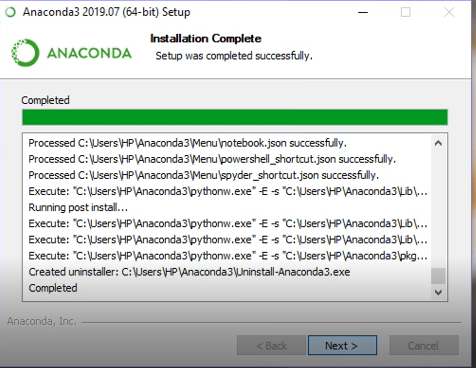
\includegraphics[scale=0.5]{figures/9}
    \caption{\textit{Installation Complete}}
    \label{Figureanaconda8}
\end{figure}

\item klik \textit{next}
\begin{figure}[H]
    \centering
    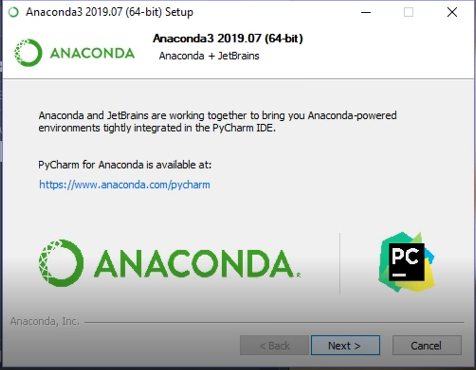
\includegraphics[scale=0.5]{figures/10}
    \caption{\textit{Anaconda+JetBrains}}
    \label{Figureanaconda70}
\end{figure}

\item Jika sudah klik \textit{finish}
 gambar \textit{Thanks fo install Anaconda}.

\begin{figure}[H]
    \centering
    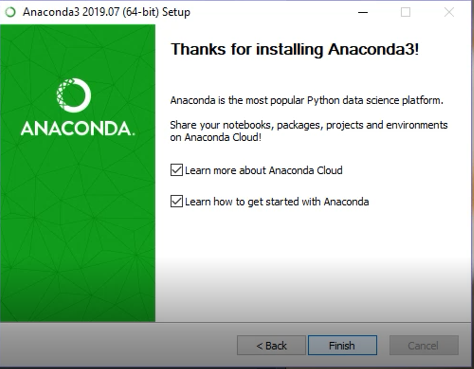
\includegraphics[scale=0.5]{figures/11}
    \caption{\textit{Thanks for install Anaconda}}
    \label{Figureanaconda70}
\end{figure}
\end{enumerate}

\section{Instalasi Pip}

\begin{enumerate}
\item buka anaconda promt
\item ketikkan Pip install selenium
\begin{figure}[H]
    \centering
    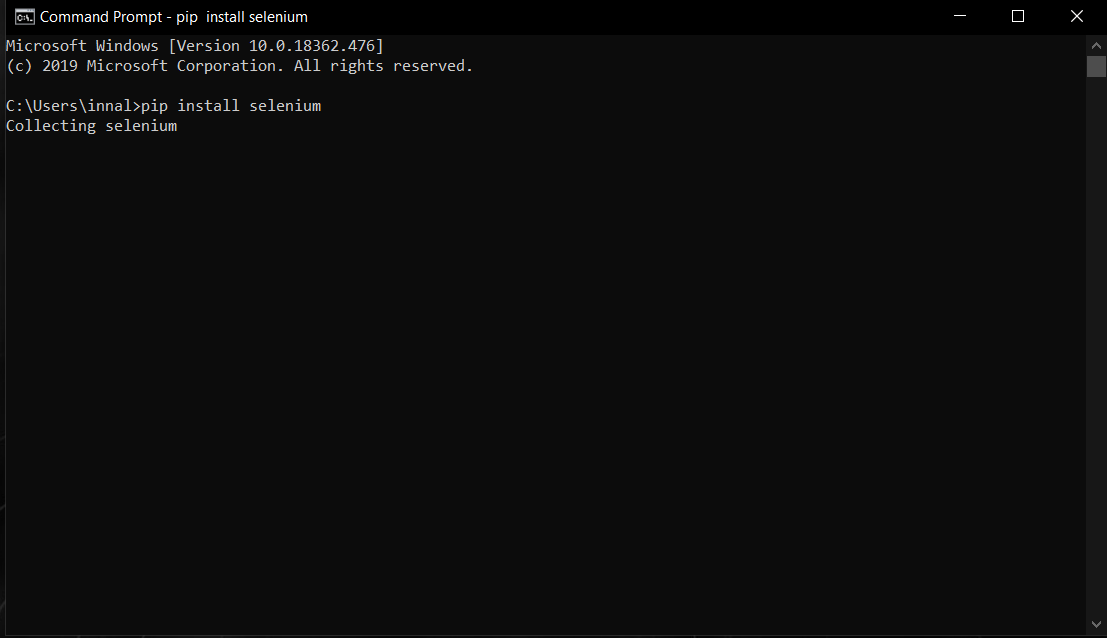
\includegraphics[scale=0.3]{figures/installpip (2)}
    \caption{\textit{Install pip}}
    \label{Figureanaconda70}
\end{figure}
\item Tunggu hingga proses instalasi selesai.
\begin{figure}[H]
    \centering
    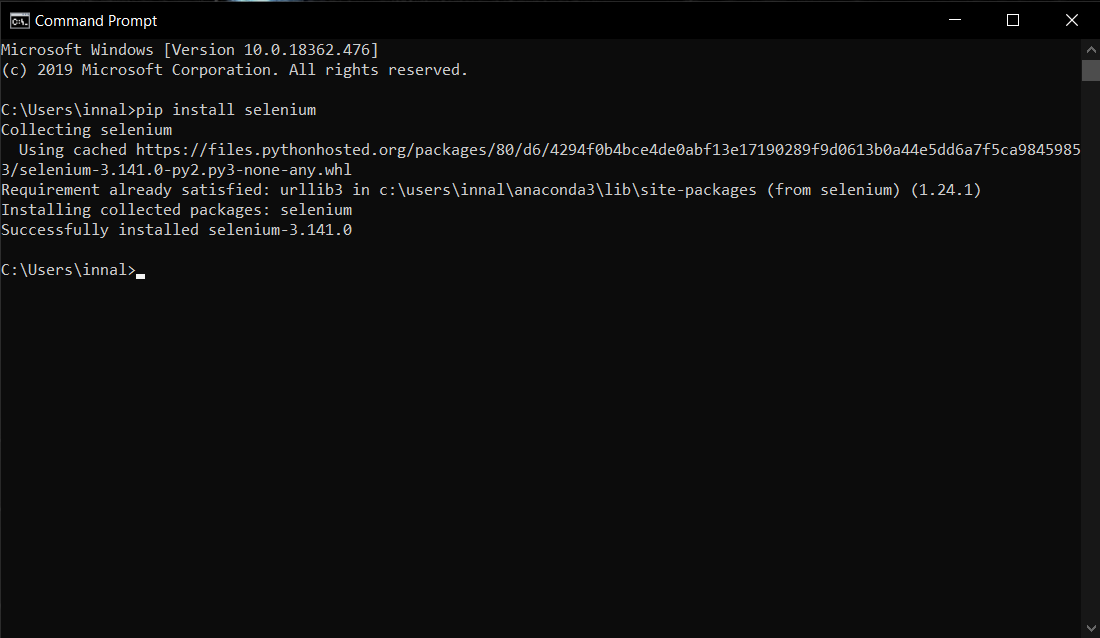
\includegraphics[scale=0.3]{figures/pipselesai (2)}
    \caption{\textit{Install pip Selesai}}
    \label{Figureanaconda70}
\end{figure}
\item jika telah selesai, lakukan pengecekan versi pip dengan mengetikkan pip -V
\begin{figure}[H]
    \centering
    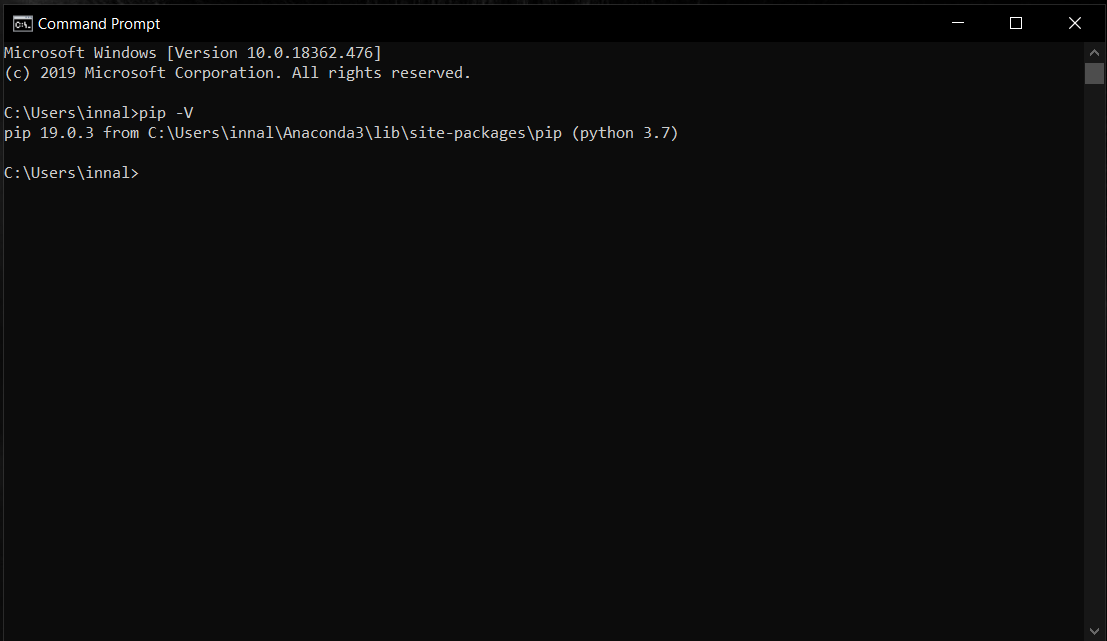
\includegraphics[scale=0.5]{figures/pipversion (2)}
    \caption{\textit{Melihat Versi pip}}
    \label{Figureanaconda70}
\end{figure}

\end{enumerate}

\section{Setting Environment}
\subsection{Windows (Windows 10)}
\begin{enumerate}
\item Buka file explorer
\item Klik kanan pada This pc, lalu pilih properties
\begin{figure}[H]
    \centering
    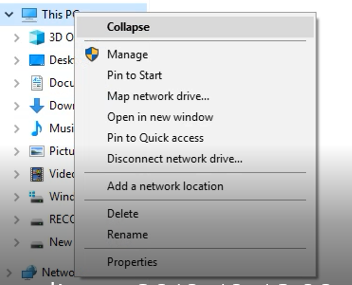
\includegraphics[scale=0.7]{figures/properties}
    \caption{\textit{Properties}}
    \label{Environment1}
\end{figure}
\item Pilih menu Advanced system settings
\begin{figure}[H]
    \centering
    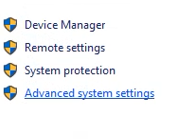
\includegraphics[scale=0.7]{figures/advanced}
    \caption{\textit{Advanced system settings}}
    \label{Environment2}
\end{figure}
\item Pilih Environment Variables
\begin{figure}[H]
    \centering
    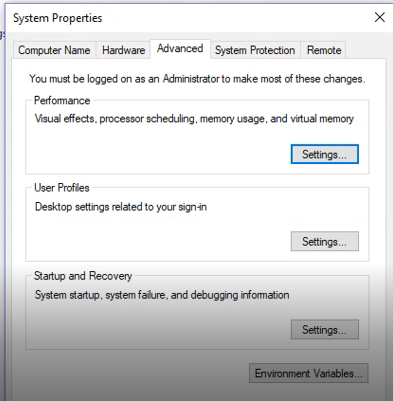
\includegraphics[scale=0.7]{figures/environment}
    \caption{\textit{Environment Variables}}
    \label{Environment3}
\end{figure}
\item Pilih Path, lalu pilih environment variable yang ingin ditambahkan, klik OK
\begin{figure}[H]
    \centering
    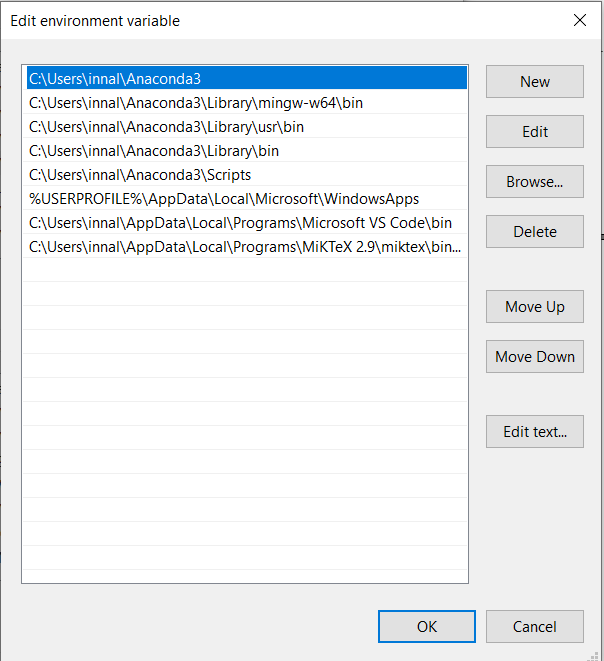
\includegraphics[scale=0.7]{figures/path}
    \caption{\textit{Path}}
    \label{Environment4}
\end{figure}

\end{enumerate}

\section{Geckodriver dan Chromedriver}
\subsection{Gechodriver untuk Mozilla Firefox}
\par Download Geckodriver pada link ini https://github.com/mozilla/geckodriver/releases. sebelum mendownload harus menyamakan versi mozilla dengan versi Geckodriver misal versi Mozilla firefox versi 32bit Geckodrivernya pun harus 32bit jika tidak maka akan terjadi kesalahan.

jika sudah mendownload Geckodriver pindahkan file tersebut ke system32
\begin{figure}[H]
    \centering
    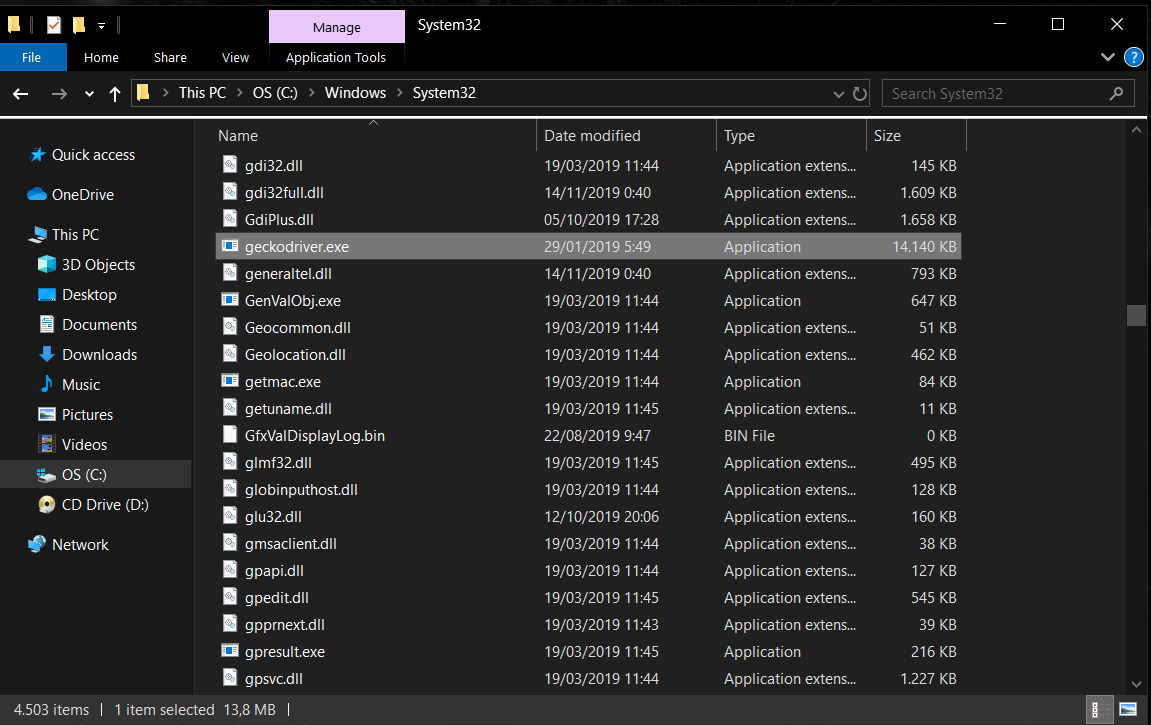
\includegraphics[scale=0.3]{figures/gechodriver}
    \caption{\textit{Gechodriver}}
    \label{Geckodriver}
\end{figure}




